\def\mytitle{PYTHON PROGRAMMING ON MATRICES}
\def\myauthor{K.Pavan Kumar}
\def\contact{r170850@rguktrkv.ac.in}
\def\mymodule{Future Wireless Communication (FWC)}


\documentclass[10pt, a4paper]{article}
\usepackage[a4paper,outer=1.5cm,inner=1.5cm,top=1.75cm,bottom=1.5cm]{geometry}

\twocolumn
\usepackage{graphicx}
\usepackage{karnaugh-map}
\usepackage{tabularx}
\usepackage{hyperref}
\usepackage[utf8]{inputenc}
\usepackage{amsmath}
\usepackage{physics}
\usepackage{amssymb}
\usepackage{watermark}
\renewcommand*\familydefault{\sfdefault}
\usepackage{lipsum}
\usepackage{xcolor}
\usepackage{listings}
\lstset{
frame=single, 
breaklines=true,
columns=fullflexible
}

\begin{document}
\thiswatermark{\centering \put(0,-110.0){
\includegraphics[scale=0.3]{logo}} }
\title{\mytitle}
\author{\myauthor\hspace{1em}\\\contact\\FWC22011\hspace{6.5em}IITH\hspace{0.5em}\mymodule\hspace{6em}Matrix:Lines}

%\{ Wireless Communication (FWC)}
\date{}
\maketitle


  \section{Problem}
In parallelogram ABCD, two points P and Q are
taken on diagonal BD such that DP = BQ. Show that: \\
(i) $\Delta APD \cong \Delta CQB$  \\       
(ii) AP = CQ\\
(iii)$\Delta AQB \cong \Delta CPD$  \\   
(iv) AQ = CP   \\
(v) APCQ is a parallelogram \\
\begin{figure}[h]
\centering
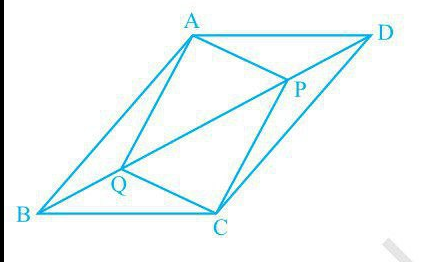
\includegraphics[scale=0.5]{ABCD.png} 
\caption{Given Figure}
\end{figure}

\section{Solution}
\begin{center}
The input parameters for this construction are
\begin{tabular}{|c|c|}
	\hline
	\textbf{Symbol}&\textbf{Value}\\
	\hline
	r&5\\
	\hline
	k&3\\
	\hline
    b&4\\
	\hline
	$\theta$&$\frac{pi}{3}$\\
	\hline
\end{tabular}
\boldmath
$$\vec{A}=\begin{pmatrix} r\cos\theta\\ r\sin\theta\ \end{pmatrix}$$
$$\vec{B}=\begin{pmatrix} 0\\ 0\ \end{pmatrix}$$
$$\vec{C}=\begin{pmatrix} b\\ 0\ \end{pmatrix}$$
$$\vec{D}={\vec{A}+\vec{C}-\vec{B}}$$
$$\vec{P} =  \frac{\vec{B} +K\times \vec{D}}{1+K}$$
$$\vec{Q} =  \frac{K\times\vec{B} +\vec{D}}{1+K}$$ 
\unboldmath
\end{center}

\textbf{Direction vectors:}
\boldmath
$$\vec{m_1}={\vec{A}-\vec{B}} $$
$$\vec{m_2}={\vec{C}-\vec{B}} $$
$$\vec{m_3}={\vec{D}-\vec{C}} $$
$$\vec{m_4}={\vec{D}-\vec{A}} $$
$$\vec{m_5}={\vec{Q}-\vec{B}} $$
$$\vec{m_6}={\vec{D}-\vec{P}} $$

$$\vec{n_1}={\vec{A}-\vec{P}} $$
$$\vec{n_2}={\vec{C}-\vec{Q}} $$
$$\vec{n_3}={\vec{A}-\vec{Q}} $$
$$\vec{n_4}={\vec{C}-\vec{P}} $$

\unboldmath
\textbf{(i)To prove:}$\Delta APD \cong \Delta CQB$  \\ 
    Distance between D and P is $\norm{\vec{D-P}}$\\
	Distance between B and Q is $\norm{\vec{B-Q}}$\\
	if $\norm{\vec{D-P}}$ =  $\norm{\vec{B-Q}}$\\
	then DP = BQ..........(1)\\

    Distance between A and D is $\norm{\vec{A-D}}$\\
	Distance between B and C is $\norm{\vec{B-C}}$\\
	if $\norm{\vec{A-D}}$ =  $\norm{\vec{B-C}}$\\
	then AD = BC..........(2)\\

	  $\angle {CBQ}$ = $\arccosine\frac{\vec{m5}^T \vec{m2}}{\norm{\vec{m5}}\norm{\vec{m2}}}$ \\
	  $\angle {ADP}$ = $\arccosine\frac{\vec{m4}^T \vec{m6}}{\norm{\vec{m4}}\norm{\vec{m6}}}$ \\
    if $\angle {CBQ}$ = $\angle {ADP}$ ........(3) \\
      From (1),(2) and (3) 
    $\Delta APD \cong \Delta CQB$  \\ 

\textbf{ii.TO prove:}AP=CQ\\
    Distance between A and P is $\norm{\vec{A-P}}$\\
	Distance between C and Q is $\norm{\vec{C-Q}}$\\
	if $\norm{\vec{A-P}}$ =  $\norm{\vec{C-Q}}$\\
	then AP = CQ..........(4)\\

\textbf{(iii)To prove:}$\Delta AQB \cong \Delta CPD$  \\ 
    Distance between D and P is $\norm{\vec{D-P}}$\\
	Distance between B and Q is $\norm{\vec{B-Q}}$\\
	if $\norm{\vec{D-P}}$ =  $\norm{\vec{B-Q}}$\\
	then DP = BQ..........(5)\\

    Distance between A and B is $\norm{\vec{A-B}}$\\
	Distance between C and D is $\norm{\vec{C-D}}$\\
	if $\norm{\vec{A-B}}$ =  $\norm{\vec{C-D}}$\\
	then AB = CD..........(6)\\
	  $\angle {ABQ}$ = $\arccosine\frac{\vec{m5}^T \vec{m1}}{\norm{\vec{m5}}\norm{\vec{m1}}}$ \\
	  $\angle {CDP}$ = $\arccosine\frac{\vec{m6}^T \vec{m3}}{\norm{\vec{m6}}\norm{\vec{m3}}}$ \\
    if $\angle {ABQ}$ = $\angle {CDP}$ ........(7) \\
      Then, from (5),(6) and (7) 
    $\Delta AQB \cong \Delta CPD$  \\ 


\textbf{iV.TO prove:}AQ=CP\\
    Distance between A and Q is $\norm{\vec{A-Q}}$\\
	Distance between C and P is $\norm{\vec{C-P}}$\\
	if $\norm{\vec{A-Q}}$ =  $\norm{\vec{C-P}}$\\
	then AQ = CP..........(8)\\

\textbf{V.APCQ is a parallelogram}\\
    From (4) and (8) ;AP=CQ and AQ=CP
    Therefore, each pair  Opposite sides are equal in quadrilateral APCQ

 	  $\angle {AQC}$ = $\arccosine\frac{\vec{n2}^T \vec{n3}}{\norm{\vec{n2}}\norm{\vec{n3}}}$ \\
	  $\angle {APC}$ = $\arccosine\frac{\vec{n1}^T \vec{n4}}{\norm{\vec{n1}}\norm{\vec{n4}}}$ \\

    $\angle {QAP}$ = $\arccosine\frac{\vec{n1}^T \vec{n3}}{\norm{\vec{n1}}\norm{\vec{n3}}}$ \\
	  $\angle {QCP}$ = $\arccosine\frac{\vec{n2}^T \vec{n4}}{\norm{\vec{n2}}\norm{\vec{n4}}}$ \\

    If $\angle {AQC}$ = $\angle {APC}$ and \\ $\angle {QAP}$ =$\angle {QCP}$ \\

    Then, each pair of  Opposite angles are equal in  quadrilateral APCQ

    \textbf{Theorem:}\\If each pair of opposite sides of a quadrilateral is equal, then it is a parallelogram. (0r) 
    If in a quadrilateral, each pair of opposite angles is equal, then it is a parallelogram.
        
    $\therefore$ Quadrilateral APCQ is a parallelogram.\\ 	

\section{Construction}
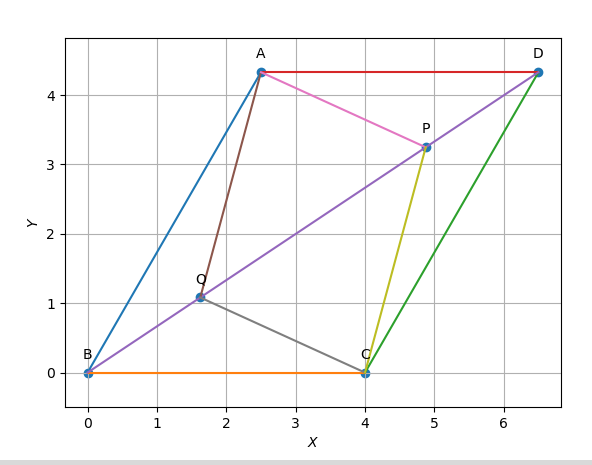
\includegraphics[scale=0.5]{construction.png} 
    
\section{Execution}
*Verify the above proofs in the following code.\\
\begin{lstlisting}
https://github.com/pavan170850/Fwciith2022/blob/main/Matrix_Lines/codes/para.py
\end{lstlisting}
	

\bibliographystyle{ieeetr}
\end{document}